%%%%%%%%%%%%
%
% $Autor: Wings $
% $Datum: 2019-03-05 08:03:15Z $
% $Pfad: Automatisierung/Skript/Produktspezifikation/Powerpoint/AMF.tex $
% $Version: 4250 $
% !TeX spellcheck = en_GB/de_DE
% !TeX encoding = utf8
% !TeX root = filename 
% !TeX TXS-program:bibliography = txs:///biber
%
%%%%%%%%%%%%

%source: https://randomnerdtutorials.com/installing-esp32-arduino-ide-2-0/

\chapter{First Steps with the Board ESP32}

Prerequisites: Arduino IDE 2 Installed

\section{Introduction}

In this chapter we will be looking at how to connect the ESP32 with a PC/laptop  in order to use the board. Then, we will be going through the first steps of installing the relevant packages to use the board ESP32 and then we will be implementing a basic example sketch from the Arduino IDE.



\section{Install ESP32 Add-on in Arduino IDE}


\Mynote{Das gesamte Kapitel muss überarbeitet werden.}


To install the ESP32 board in your Arduino IDE, follow these next instructions:

\begin{enumerate}
  \item In your Arduino IDE 2, go to \menu{File > Preferences}.
    
    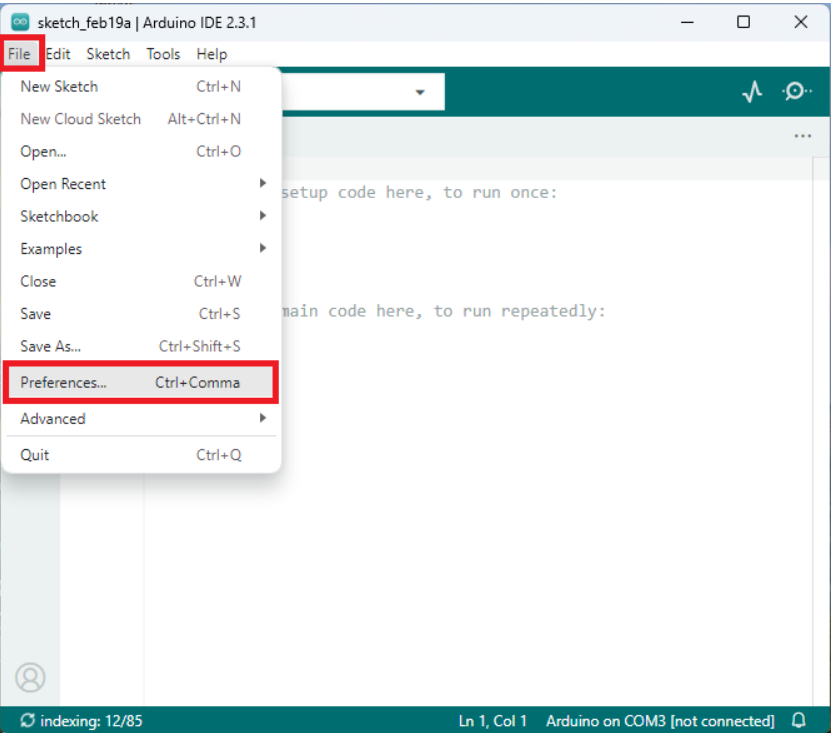
\includegraphics[width=0.8\textwidth]{ESP32/ArduinoIDE/Preferences}
    
  \item Copy and paste the following line to the Additional Boards Manager URLs field.
  
        \medskip
  
        \URL{https://raw.githubusercontent.com/espressif/arduino-esp32/gh-pages/package_esp32_index.json}
  
        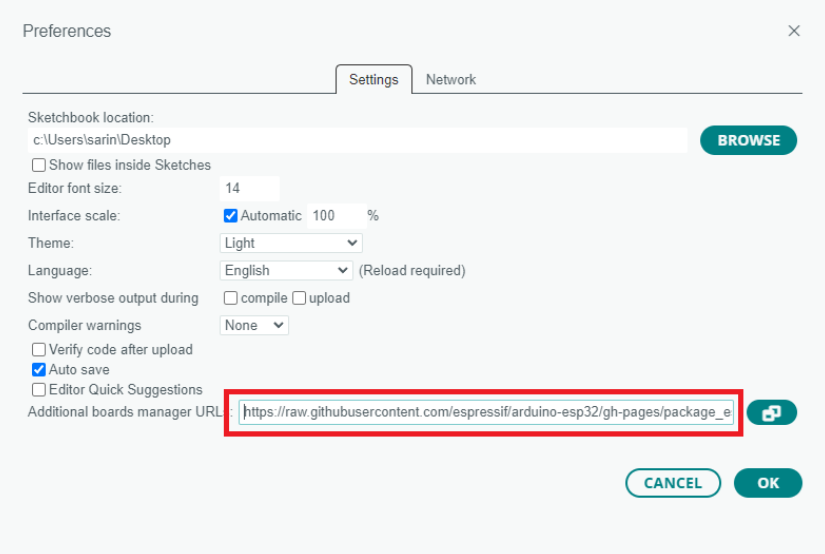
\includegraphics[width=0.8\textwidth]{ESP32/ArduinoIDE/PreferencesDialogue}
  
        \medskip
          
        Note: if you already have the ESP8266 boards URL, you can separate the URLs with a comma, as follows:
  
        \medskip
       
       \URL{http://arduino.esp8266.com/stable/package_esp8266com_index.json}, \URL{https://raw.githubusercontent.com/espressif/arduino-esp32/gh-pages/package_esp32_index.json}
       
  \item Open the Boards Manager. You can go to \menu{Tools > Board > Boards Manager\ldots} or you can simply click the Boards Manager icon in the left-side corner.       
  
        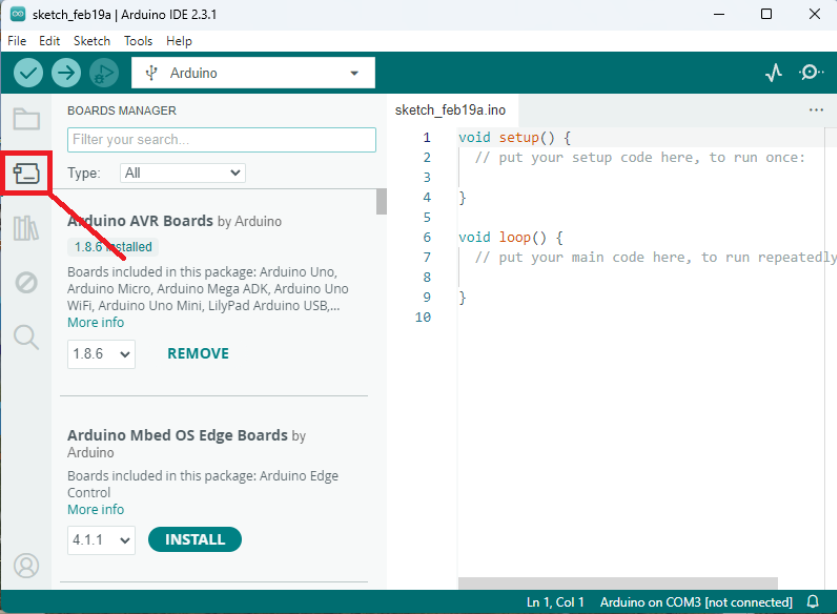
\includegraphics[width=0.8\textwidth]{ESP32/ArduinoIDE/BoardManager}
        
  \item Search for \textbf{ESP32} and press the install button for \textbf{esp32 by Espressif Systems}.        
  
        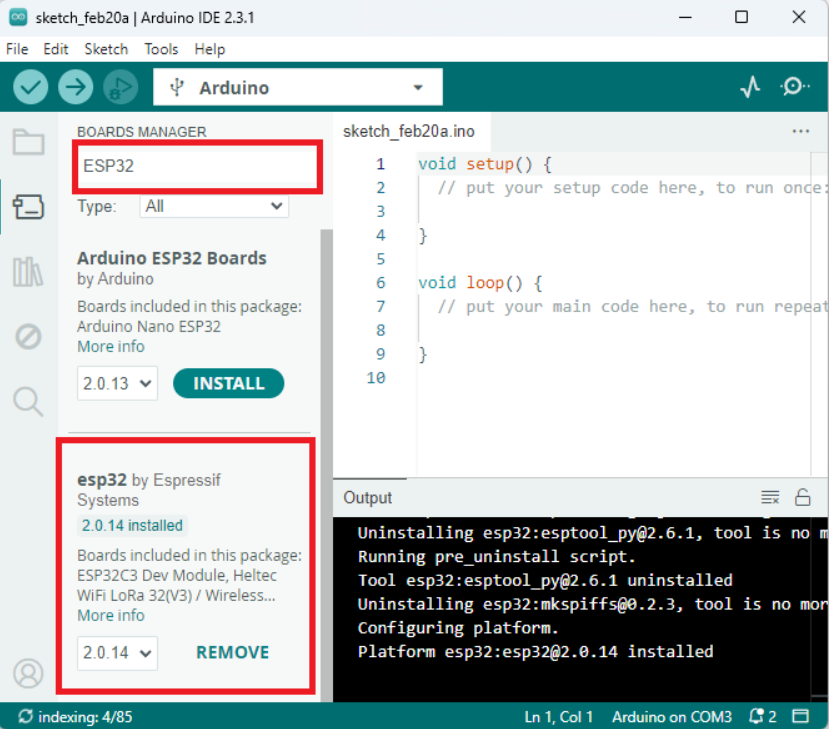
\includegraphics[width=0.8\textwidth]{ESP32/ArduinoIDE/BoardManagerESP32}
  
\end{enumerate}

\medskip

That's it. It should be installed after a few seconds.

\section{Testing the Installation}

\subsection{Loading the sketch \FILE{TestBuiltinLED.ino}}

To test the ESP32 add-on installation, we’ll upload a simple code that blinks the on-board LED (GPIO 2).

\medskip

Copy the following code to your Arduino IDE:

{
    \captionof{code}{Simple sketch to control the built-in LED}\label{ESP32:BuiltinLEDTest}
    \ArduinoExternal{}{../../Code/ESP32/Test/TestLEDBuiltin.ino}
}


\subsection{Uploading the Sketch}

Select your board before uploading the code. On the top drop-down menu, click on \menu{Select other board and port\ldots}

        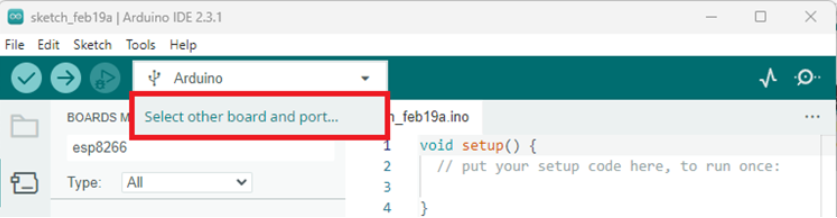
\includegraphics[width=0.8\textwidth]{ESP32/ArduinoIDE/Port}
        
A new window, as shown below, will open. Search for your ESP32 board model.

        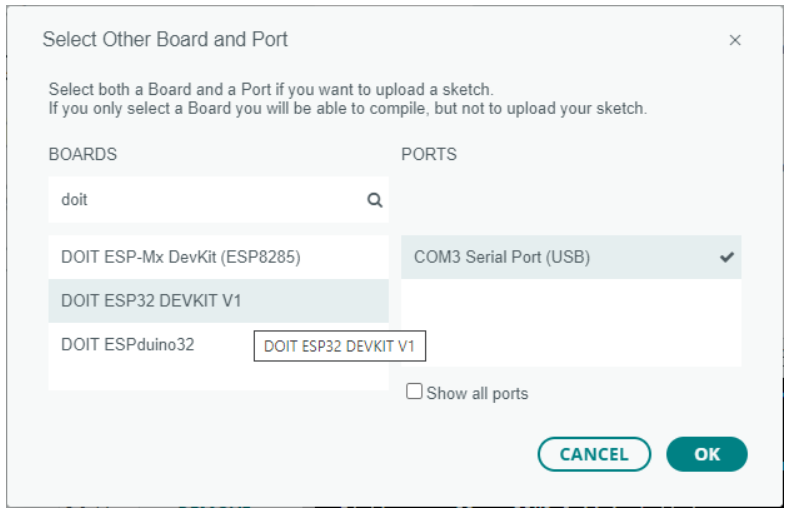
\includegraphics[width=0.8\textwidth]{ESP32/ArduinoIDE/BoardAndPort}
        
Select the ESP32 board model you're using, and the COM port. In our example, we're using the DOIT ESP32 DEVKIT V1. Click \textbf{OK} when you're done.

\bigskip

Now, you just need to click on the Upload button.        
        

        
\includegraphics[width=0.2\textwidth]{ESP32/ArduinoIDE/Upload}
        
After a few seconds, the upload should be complete.        

        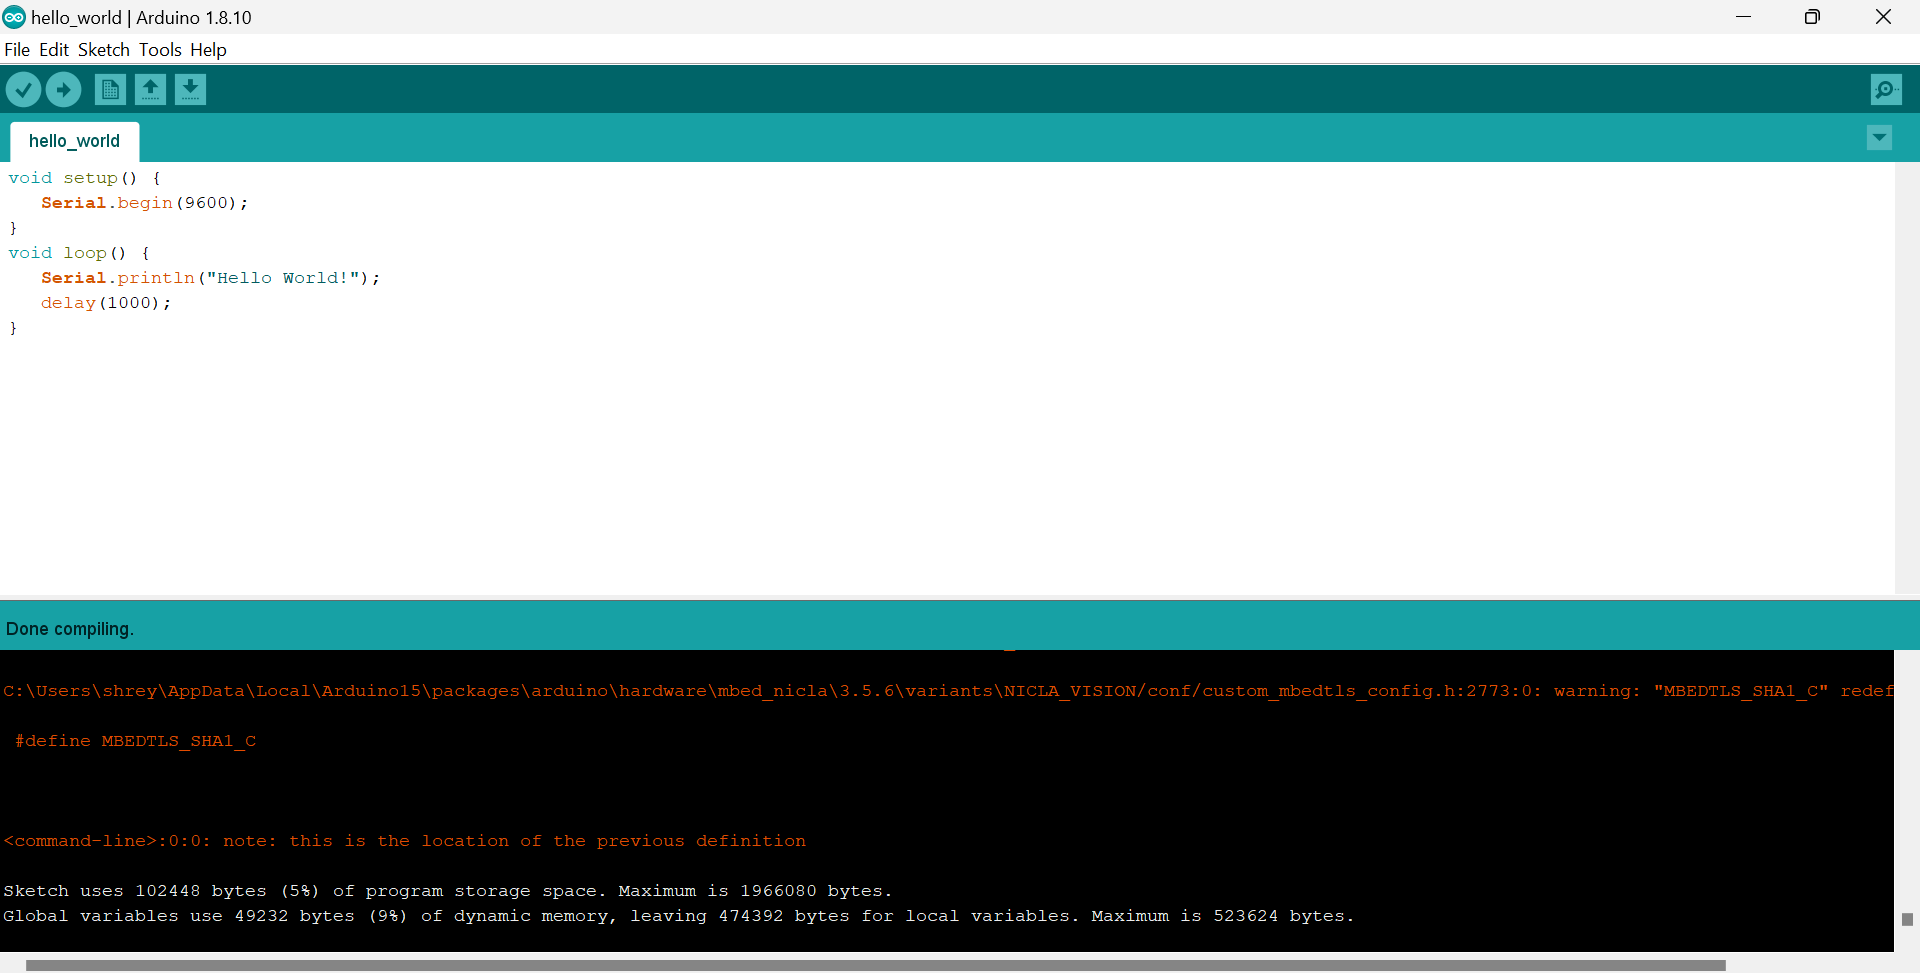
\includegraphics[width=0.2\textwidth]{ESP32/ArduinoIDE/HelloWorld}
        
Note: some ESP32 development boards don’t go into flashing/uploading mode automatically when uploading a new code and you’ll see a lot of dots on the debugging window followed by an error message. If that’s the case, you need to press the ESP32 BOOT button when you start seeing the dots on the debugging window.

\bigskip

The ESP32 on-board LED should be blinking every second.        

        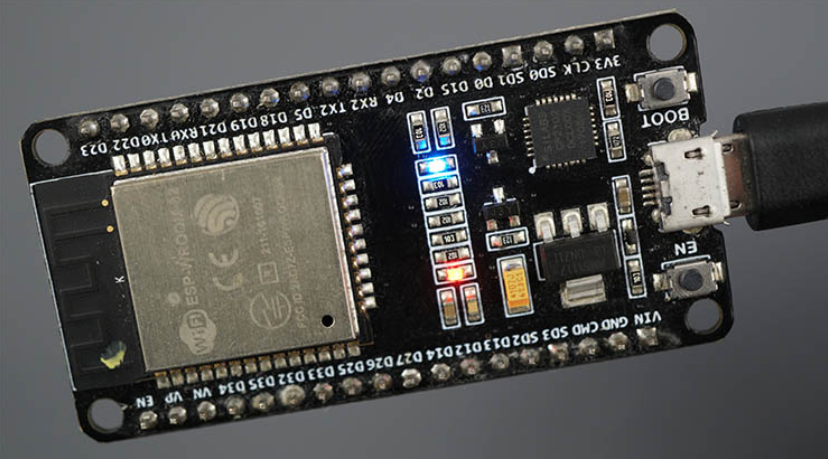
\includegraphics[width=0.8\textwidth]{ESP32/ArduinoIDE/HWBlink}
        
\subsection{Serial Monitor}

You can click on the Serial Monitor icon to open the Serial Monitor tab. Make sure you select the 115200 baud rate.        

        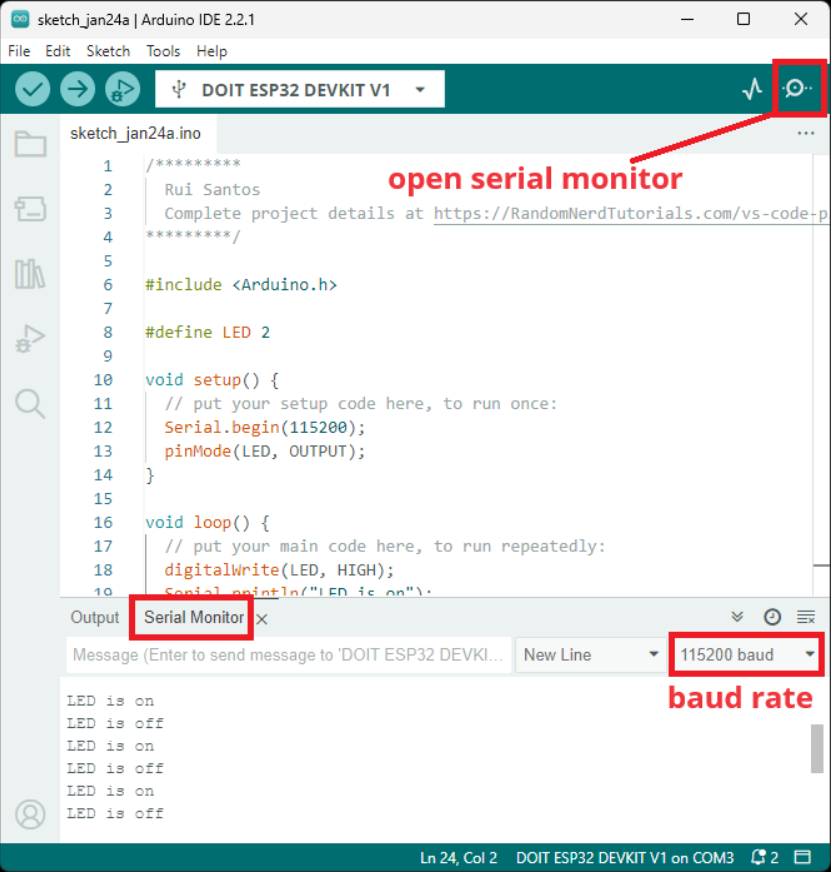
\includegraphics[width=0.8\textwidth]{ESP32/ArduinoIDE/SerialMonitor}

\section{Troubleshooting}


\begin{enumerate}
  \item If you try to upload a new sketch to your ESP32 and you get this error message ``A fatal error occurred: Failed to connect to ESP32: Timed out\ldots Connecting\ldots''. It means that your ESP32 is not in flashing/uploading mode.

  \bigskip
  
  Having the right board name and COM por selected, follow these steps:
  
  \begin{itemize}
    \item Hold-down the BOOT button in your ESP32 board
    \item Press the Upload button in the Arduino IDE to upload your sketch
    \item After you see the  message ``Connecting\ldots'' in your Arduino IDE, release the finger from the button BOOT
    \item After that, you should see the message ``Done uploading''
  \end{itemize}


  \medskip
  
  You'll also have to repeat that button sequence every time you want to upload a new sketch. But if you want to solve this issue once for all without the need to press the button BOOT, follow the suggestions in the next guide:

  \begin{itemize}
    \item \HREF{https://randomnerdtutorials.com/solved-failed-to-connect-to-esp32-timed-out-waiting-for-packet-header/}{[SOLVED] Failed to connect to ESP32: Timed out waiting for packet header}
  \end{itemize}

  \item  If you get the error ``COM Port not found/not available'', you might need to install the CP210x Drivers:

  \begin{itemize}
    \item \HREF{https://randomnerdtutorials.com/install-esp32-esp8266-usb-drivers-cp210x-windows/}{Install USB Drivers – CP210x USB to UART Bridge (Windows PC)}
    \item \HREF{https://randomnerdtutorials.com/install-esp32-esp8266-usb-drivers-cp210x-mac-os/}{Install USB Drivers – CP210x USB to UART Bridge (Mac OS X)}
  \end{itemize}

\end{enumerate}


If you experience any problems or issues with your ESP32, take a look at our in-depth \HREF{https://randomnerdtutorials.com/esp32-troubleshooting-guide/}{ESP32 Troubleshooting Guide}.

\section{ESP32 Filesystem Uploader Plugin}

After installing the ESP32 boards on the Arduino IDE 2, you may also want to install the filesystem uploader plugin to easily upload files to the ESP32 filesystem (LittleFS)—check the following tutorial:

  \begin{itemize}
    \item \HREF{https://randomnerdtutorials.com/arduino-ide-2-install-esp32-littlefs/}{Arduino IDE 2: Install ESP32 LittleFS Uploader (Upload Files to the Filesystem}
  \end{itemize}
    